Iterating over a set of ideas is an intrinsic part of both the
\emph{Engineering Design Process} and research, and some end being discarded.
Nevertheless, knowing about the discarded paths can be helpful~\cite{conroy_three_2020}
since they can point to either future lines of work or dead-ends not worth pursuing.

In this appendix, we briefly describe one insight and two prototypes generated during
the development of this thesis that did not prove successful.

\section{Types of Data Correlation}

In 2017, \cite{Kraska2017} proposed a novel idea: an index over a dataset
is just a model. This model takes as input a value, or a range of values,
and ``predicts'' the physical location of the corresponding tuples.
In this work, Kraska \etal propose \emph{learned} alternatives to well-known data
structures often used on databases for different access patterns:
value range (typically modeled with B-trees), unique values (hash tables),
and existence queries (Bloom filters).
However, Kraska \etal trained models over a single attribute.
Extending these types of models might also be possible when multiple files exist.

Thus, based only on the data, we can learn models to predict the value of
attributes related to the physical layout, such as the file where a tuple is contained and its offset.
This is possible under the assumption that there are three types of \emph{correlations}
or \emph{dependencies}:

\begin{itemize}
    \item \textbf{File Correlation} Dependence between values and containing file.
    \item \textbf{Offset Correlation} Dependence between values and offset within the
        file~\cite{Kraska2017}.
    \item \textbf{Tuple Correlation} Dependence between the attribute values of a tuple.
\end{itemize}

Note that the first two correlations depend on the acquisition method and the third
on the measured properties.

\PresQ builds on the third assumption in order to find \glspl{EDD}: same set of attributes
from the same population follow the same distribution.

We now describe an attempt to leverage the first type of correlation in
section~\ref{sec:file_correlation}, a naive indexing approach on section~\ref{sec:offset_correlation},
and an early prototype for schema matching in section~\ref{sec:attribute_correlation}.

\section{File Correlation}
\label{sec:file_correlation}

Large datasets may be partitioned into multiple files to facilitate their use.
This partitioning can be done as a function of some data features: spatial coordinates,
alphanumerical order, temporal order, etc. Therefore, machine learning techniques
should be able to model (index) this partitioning without user intervention.

As a proof-of-concept, we took two astronomical catalogs partitioned into multiple
files generated by two different processes: simulation and measurement.

We can see the indexing as a ``classification'' task: we want to model the file
corresponding to a given data set. For the feature selection, we use Random Forest
with 100 trees. Features with higher weight are those used to partition the data.
Code~\ref{code:sel_attr_multifile} shows a snippet of the feature selection.
We executed it over a random sample of 5000 tuples per file.
We obtained that the sky coordinates --- right ascension and declination --- were
the best features for both the simulation and the measurement catalogs.

\begin{listing}[H]
\begin{minted}[linenos]{python}
# feat_cols contains all features except the file index
classifier = RandomForestClassifier(n_estimators = 100)
classifier.fit(train[feat_cols], train['FILE'])
# Contains the weight for each feature
classifier.feature_importances_
\end{minted}
\caption{Feature selection for file correlation}
\label{code:sel_attr_multifile}
\end{listing}

Since trees are a data structure commonly used for spatial partitioning
--- KD-Tree, Binary Partition Tree, R-Tree --- we trained two decision trees over
both catalogs using the sky coordinates as features.
We display the resulting ``learned'' partitioning over the actual data distribution
in figure~\ref{fig:tree_cat_cut}.
We can see that in the simulated catalog, the prediction is very accurate.
However, the results are suboptimal over the real-world catalog due to overlapping catalogs.
This issue could be fixed by training a binary classifier by file.

\begin{figure}[htbp]
    \begin{subfigure}[]{0.5\textwidth}
    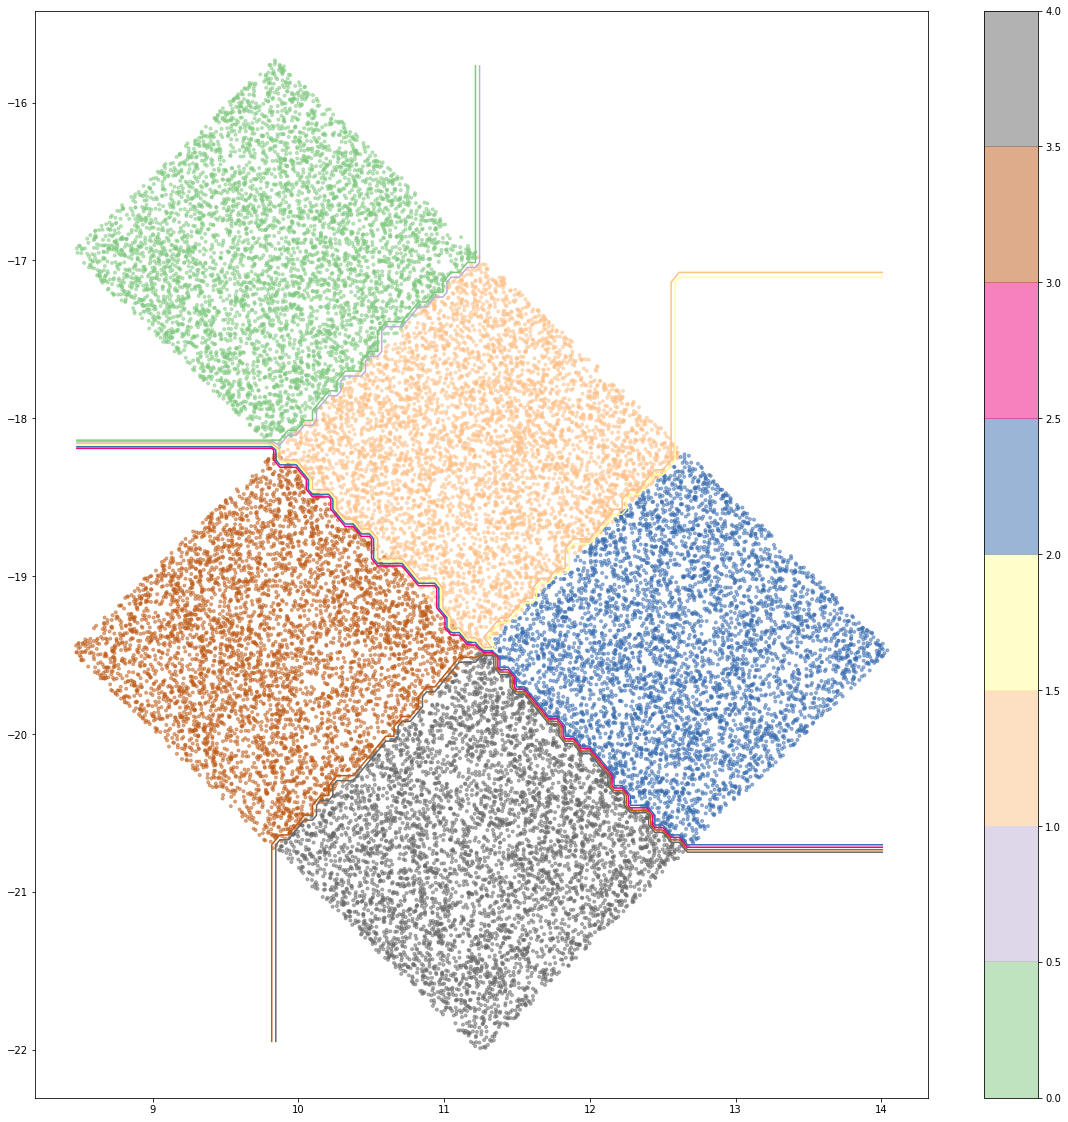
\includegraphics[width=\textwidth]{images/A2_prototypes/tu_multifile_tree.png}
    \caption{Without overlap}\label{subfig:tu_multifile}
    \end{subfigure}
    \hfill
    \begin{subfigure}[]{0.5\textwidth}
    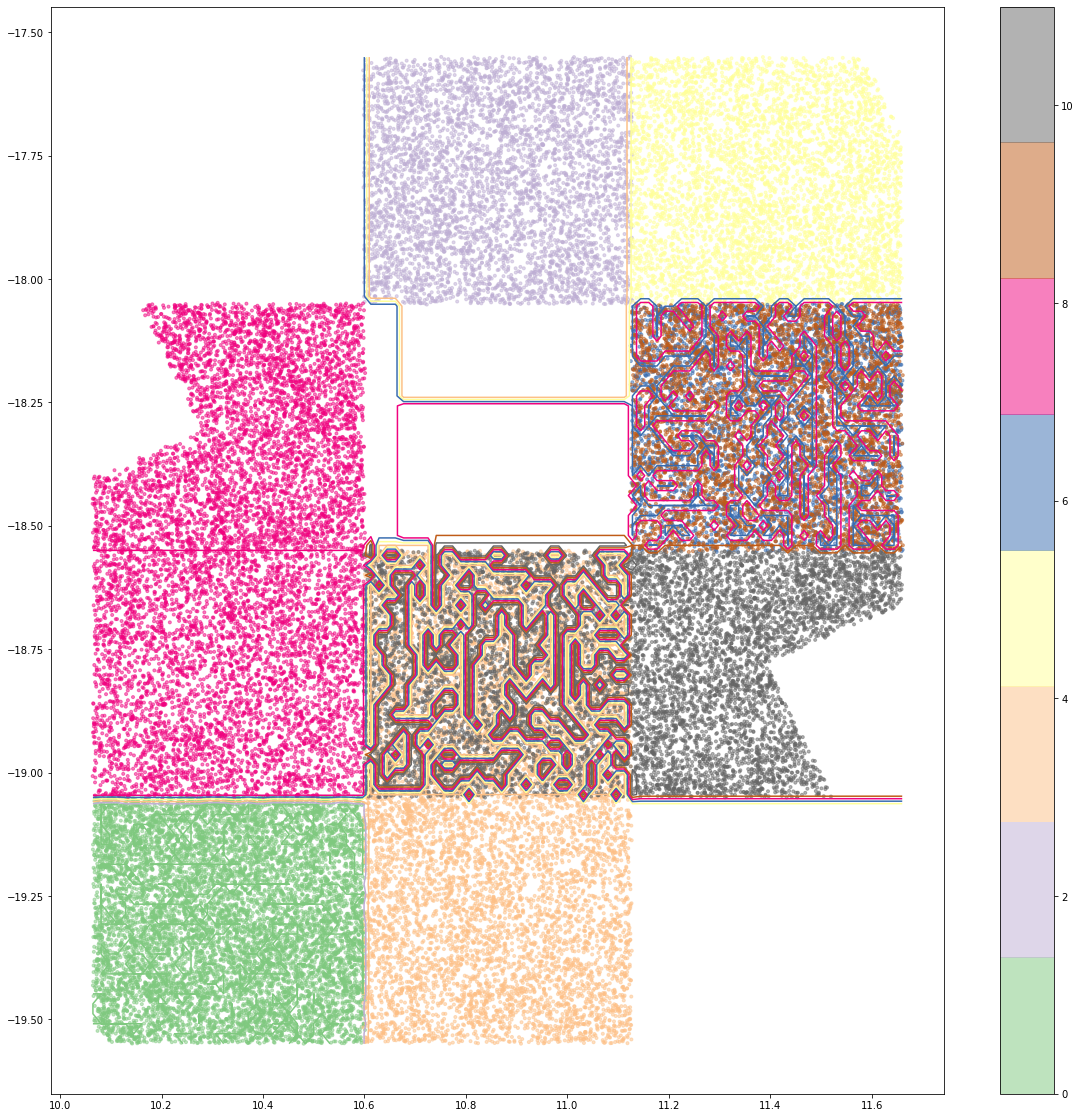
\includegraphics[width=\textwidth]{images/A2_prototypes/mer_multifile_tree.png}
    \caption{With overlap}\label{subfig:mer_multifile}
    \end{subfigure}
    \caption[Data sets distributed multiple files based on two spatial coordinates.]{
        Data sets distributed multiple files based on two spatial coordinates.
        Each color corresponds to a single file.
    }
    \label{fig:tree_cat_cut}
\end{figure}


\section{Offset Correlation}
\label{sec:offset_correlation}

We work with the assumption that the data acquisition method influences
the data distribution within a file containing raw data.

To validate the idea, we obtain random samples from three astronomical catalogs
(\gls{Cosmos}\cite{laigle2016cosmos2015}, \gls{SDSS}\cite{SDSS14}, and \gls{KiDS}\cite{de2013kilo}),
all extracted from the same sky region.

As for the file correlation case, the best features are sky coordinates.
The target variable is the page offset within the file, which we obtained via code~\ref{code:page}.
Rather than training a simple regression model and predicting the exact page, we trained models
capable of predicting a page range: \textit{Quantile Regression Forests}~\cite{meinshausen2006}
and \textit{Gradient Boosting}~\cite{mason2000}.
The training set comprises 10\% of the tuples (1\% for Cosmos, given its size) and the test
set 20\% of the remaining tuples.

The same test were run over a non astronomical data-set\footnote{\url{https://www.kaggle.com/sobhanmoosavi/us-accidents}}, for which
the best features are \texttt{Start\_Time}, \texttt{End\_time} and
\texttt{Weather\_Timestamp}\footnote{\texttt{ID} is a better feature, but trivial.}.

\begin{listing}[htpb]
\begin{minted}[linenos]{python}
block_size = os.statvfs("/path/to/files").f_bsize
row_size = np.array(table[0:1]).nbytes
page = (np.arange(len(table)) * row_size) // block_size
\end{minted}
\caption{Computation of the page offset}
\label{code:page}
\end{listing}

Table~\ref{tab:offset_prediction} summarizes the results of both models
for the four datasets. \textit{Quantile Regression Forests} can be accurate --- it predicts
the correct range --- but the overhead is not negligible --- it needs to read
a considerable portion of the file per prediction.

\begin{table}[htpb]
    \begin{tabularx}{\linewidth}{X l c r r r}
    \thead{Catalog} & \thead{N.Pages} & \thead{Method} &
    \thead{Time (s)} & \thead{Accuracy} & \thead{Precision}\\
    \hline

    \multirow{2}{*}{Cosmos} & \multirow{2}{*}{78 499} &
        QRF &  16.69 & 94.30\% & 99.61\% (306) \\
    & & GB  & 128.07 & 63.30\% & 98.43\% (1236)  \\

    \hline

    \multirow{2}{*}{SDSS} & \multirow{2}{*}{1 825} &
        QRF &  6.86 & 95.74\% & 93.47\% (119) \\
    & & GB  & 21.28 & 60.73\% & 96.85\% (57) \\

    \hline

    \multirow{2}{*}{KiDS} & \multirow{2}{*}{7 773} &
        QRF &  8.62 & 97.37\% & 99.64\% (28) \\
    & & GB  & 41.22 & 62.33\% & 98.37\% (127) \\
    
    \hline
    
    \multirow{2}{*}{Accidents} & \multirow{2}{*}{261 193} &
        QRF &127.56 & 84.86\% & 80.89\% (49926) \\
    & & GB  &  9.13 & 61.00\% & 85.90\% (36820) \\
    
    \end{tabularx}
    \caption[QR vs GBR over different datasets.]{
    QR vs GBR over different datasets.
    \emph{Time}: Training time
    \emph{Accuracy}: Ratio of predicted ranges that contain the queried tuple.
    \emph{Precision}: 1 - (Average predicted range size divided by the total file size).}
    \label{tab:offset_prediction}
\end{table}


\section{Attribute Correlation}
\label{sec:attribute_correlation}

Within a relation, we expect some attributes to be closely correlated.
This correlation is inherent to the attributes and the sampled population.
Thus, two files containing samples for the same attributes from the same
underlying population should have a similar distribution.

This correlation is intrinsic to the data and independent of the physical
schema of the data --- i.e., file layout or attribute names. Alternatively,
two datasets with different schemas but containing a similar subset of
measures should show the same dependencies between attributes. We can
expect to use these dependencies to match schemas\footnotemark.

\footnotetext{This insight directed the research toward the Equally-Distributed-Dependencies.}

Since Bayesian networks~\cite{pearl1988}  model the data dependencies
as a directed acyclic graph, we can expect that graphs trained over different
datasets containing the same information should contain isomorphic sub-graphs.

For validating the idea, we have trained three Bayesian networks using\linebreak
\textsc{Pomegranate}~\cite{schreiber2018pomegranate} over the catalogs
\gls{SDSS}, \gls{KiDS} and \gls{Cosmos}. Figure~\ref{fig:bayes1} shows the
resulting graphs for the first two, and figure~\ref{fig:bayes2} for the last.

These graphs are significantly similar for \gls{SDSS} and \gls{KiDS},
even on the order of the bands. This match is less evident for \gls{Cosmos},
given the different bands present in the catalog. However, the correspondence is
remarkable if we consider the physical order of the bands --- shown in table~\ref{tab:bandas}.

However, there remain two problems:

Most existing algorithms do not support learning Bayesian networks over continuous features,
and it is necessary to discretize them first. If this approach is not enough, there are some
proposals to train Bayesian networks using a combination of continuous and discrete
variables~\cite{Lucas2015,chen2017}.

There needs to be more than the correspondence between nodes in the graphs to compute
the correspondence between attributes. The Bayesian networks may not be stable, with
attributes changing relative positions or relations being missed.

\begin{figure}[htpb]
    \centering
    \begin{subfigure}[]{\textwidth}
    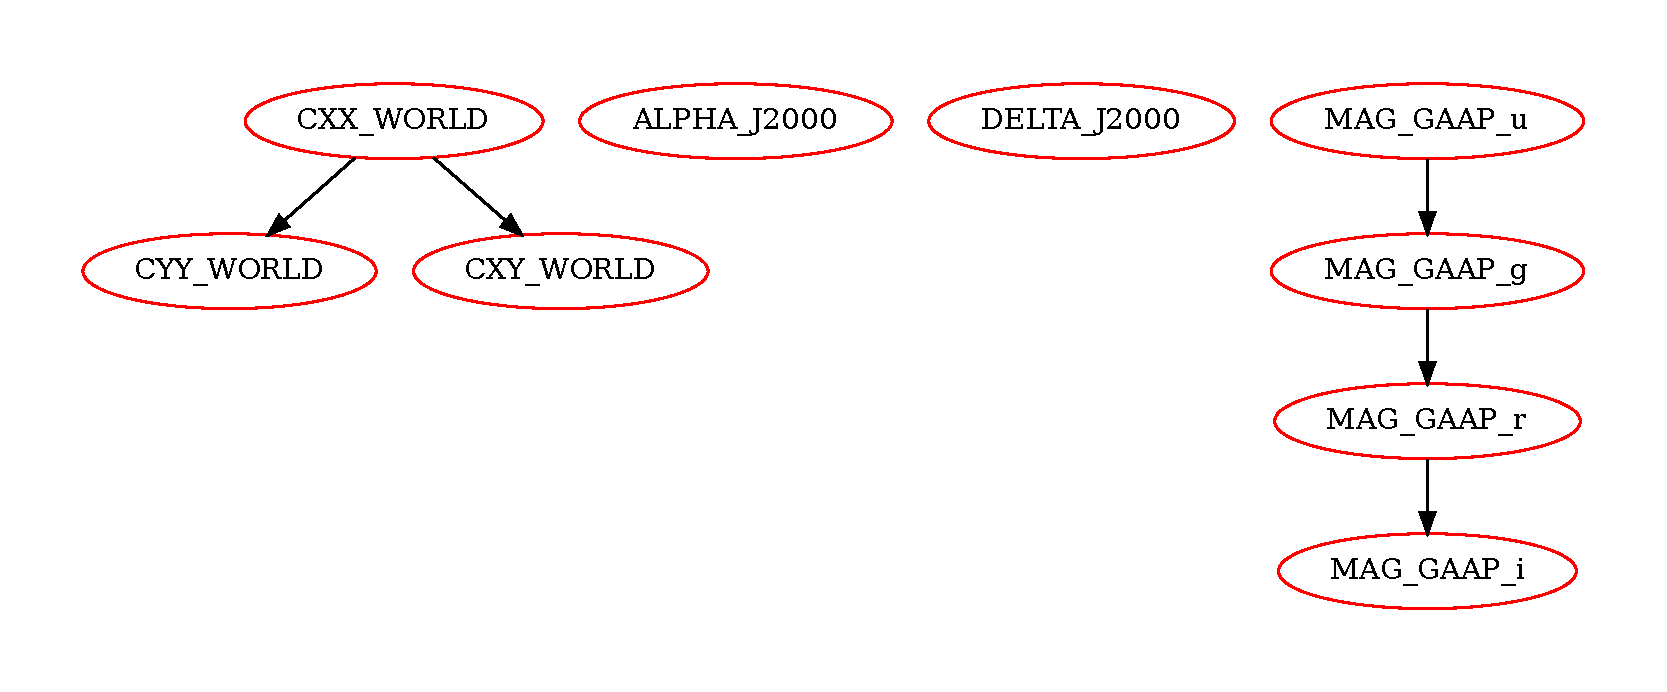
\includegraphics[width=\textwidth]{images/A2_prototypes/png_kids.pdf}
    \caption{\gls{KiDS}}
    \end{subfigure}
    \begin{subfigure}[]{0.5\textwidth}
    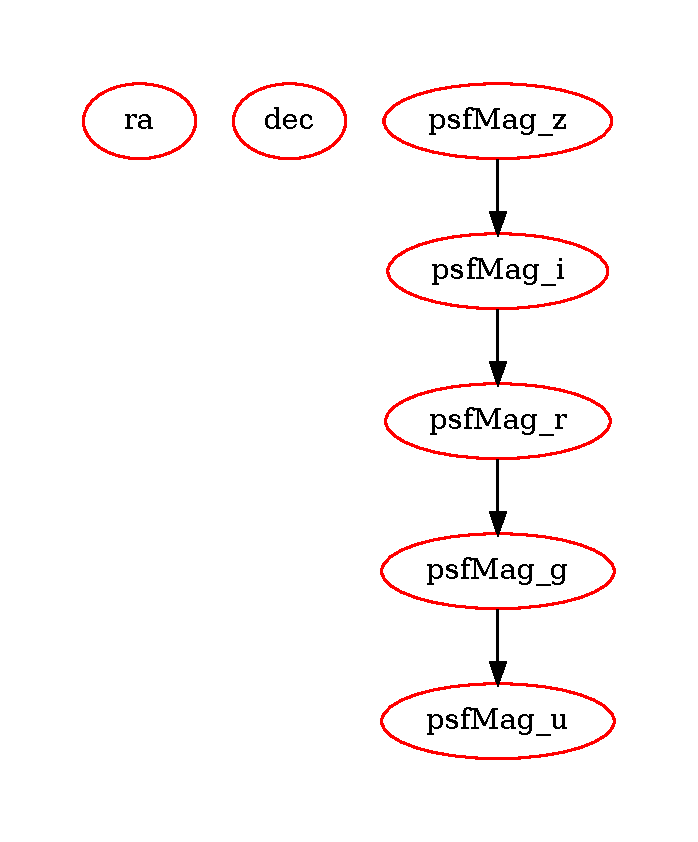
\includegraphics[width=\textwidth]{images/A2_prototypes/png_sdss.pdf}
    \caption{\gls{SDSS}}
    \end{subfigure}
    \caption{Two \glsfmtplural{PGN} trained over two different astronomical catalogs.}
    \label{fig:bayes1}
\end{figure}

\begin{figure}[htpb]
    \centering
    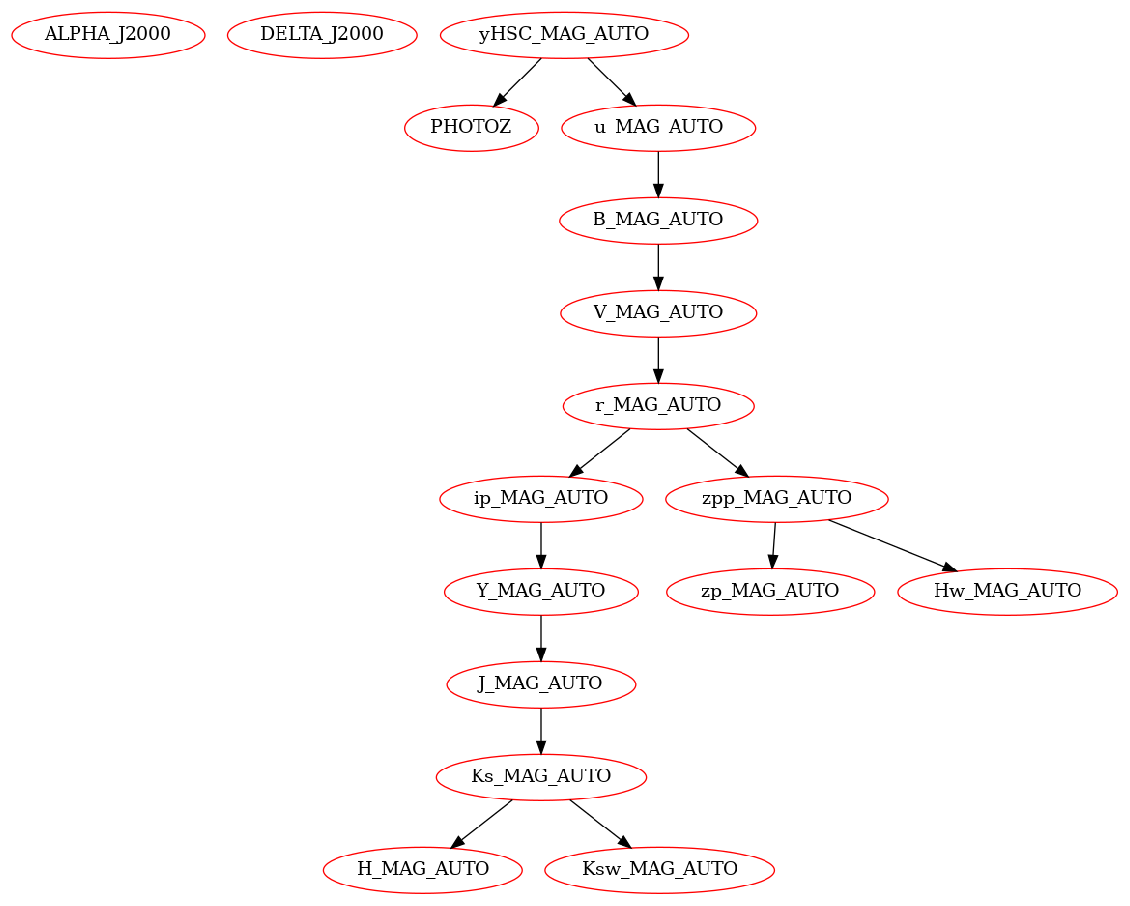
\includegraphics[width=\textwidth]{images/A2_prototypes/cosmos_bayes.png}
    \caption{\glsfmtlong{PGN} trained over \glsfmtshort{Cosmos}.}
    \label{fig:bayes2}
\end{figure}

\begin{table}[htpb]
    \begin{tabularx}{\textwidth}{c c c X c}
        \textbf{Bands} & \textbf{$\lambda$} &
        \textbf{\glsxtrshort{FWHM}} & \textbf{Filters} & \textbf{Description} \\ \hline
        \multicolumn{5}{c}{\textbf{Ultraviolet}} \\ \hline
        U & 365 nm & 66 nm  & u, u', u*             & \\
        \multicolumn{5}{c}{\textbf{Visible}} \\ \hline
        G & 464 nm & 128 nm & g'                    & Green \\
        R & 658 nm & 138 nm & r, r', R', Rc, Re, Rj & Red \\
        \multicolumn{5}{c}{\textbf{Near Infrared}} \\ \hline
        I & 806 nm  & 149 nm & i, i', Ic, Ie, Ij     & Infrared \\
        Z & 900 nm  &        & z, z'                 & \\
    \end{tabularx}
    \caption[Subset of electromagnetic bands.]{
    \href{https://en.wikipedia.org/wiki/Photometric_system}{Subset of
            electromagnetic bands}. $\lambda$ corresponds to the wavelength.}
    \label{tab:bandas}
\end{table}
